%% ------------------------------------------------------------------------- %%
\chapter{Evaluations, Results, and Discussion}
\label{cap:evaluations}
 
 \epigraph{
 	Buy it, use it, break it, fix it,\\
 	Trash it, change it, mail - upgrade it,\\
 	Charge it, point it, zoom it, press it,\\
 	Snap it, work it, quick - erase it..\\
 	..\\
 	Technologic. Technologic.}
 {Daft Punk}



%%MQZ: Aqui tem MUITA repetição do capítulo de metodologia! Estou eliminando as redundâncias, mas a fluência do texto será prejudicada...
%% Também não faz sentido no seu capítulo de resultados apresentar resultados de outros (isso fica em "trabalhos relacionados", não aqui...)
%\paragraphdesc{motivation based on experiences from compmus and nusom}
%Currently I am a member of Computer Music Research Group~(Compmus) from Universidade de São Paulo, and this group is a partner of the Research Centre on Sonology~(NuSom) from the same university.
%Recent projects and performances at the Compmus and NuSom research groups have used technologies for music interaction for short and long range distances.
%Scientists and musicians were working together in order to create multimedia environments for musical performances using local networks and the Internet.
%As this research unfolded, mobile devices have reached a comparable level of computation power with respect to desktop computers, having their mobility also improved by advances in network technologies such as the development of 4G and faster WiFi standards.
%The projects from the group and the advances in mobile technologies during the 2010's encouraged the development of this research in the field of music and mobile networks, or better saying in MM.

%\paragraphdesc{group results}
%The past researches decided to transmit audio between devices locally connected or through the Internet, but some researchers were the main inspiration for this work.
%As previously discussed, \citefullauthor{Schiavoni2013thesis} developed Medusa, a distributed audio environment~\cite{Schiavoni2013thesis} that allows users to interconnect using several  network protocols for audio and MIDI exchange.
%The protocols implemented were UDP, TCP, DCCP, and SCTP while the audio transmitted was configured to 44.1~kHz and 16~bits that would require a network bandwidth of almost 700~kbps for each audio channel.
%Many evaluations were conducted in different scenarios for LAN intercommunication, with latency varying from 0.13~ms to 72.06~ms, jitter varying from 0.08~ms to 166.49~ms, and packet loss up to 7.065\%.
%%MQZ: o Marcio não fez avaliações de comunicação em rede.
%Another research is \citefullauthor{Tomiyoshi2013thesis}, who developed the JackTripMod, a flexible and easy-to-use alternative for network music performances~\cite{Tomiyoshi2013thesis}.
%As modification of the JackTrip, this project includes a lossy compression using CELT~\cite{Valin2010high}, which is an efficient and low latency solution for encoding audio before transmitting over the network.
%This project shows that 93~kbps is the bandwidth required for transmitting an audio with 48~kbps of compression quality through the JackTripMod, in comparison with the 128~kbps required by the SoundJack~\cite{Carot2009musical} at the same setting and the 28~kbps by Skype~\cite{Skype2017} with an unknown configuration.
%Their results show that some protocols have good performance for local audio transmission in local networks, and audio transmission with lossy compression and high quality is possible depending on the network bandwidth available.
%High quality audio transmission through a large bandwidth can be considered a problem at some contexts and the addition of delays to permit this high quality may be another problem as well.

%%MQZ: As duas frases abaixo têm cara de introdução
%Although mobile devices present wireless connection as an alternative to wired solutions, the bandwidth of new wireless standards is quite comparable to wired options.
%Additionally, new mobile devices present multicore processors and optimized operating systems that surpass previous devices settings and drawbacks from old systems regarding the audio stack.

\paragraphdesc{description of our evaluation: data transmission over long distance}
The context of the evaluations in this chapter follows the proposals and results from past researches from Compmus group members, including some other assumptions.
\paragraphdesc{audio synthesis in realtime on mobile devices}
In the beginning of my research I collaborated with a project by \citefullauthor{bianchi2014processamento}, in which he evaluated realtime DSP on Android devices.
Together we explored the advantages of using JNI instead of pure Java with results described in \citep{deCarvalhoJunior2013fftbenchmark}.
In his thesis, \citefullauthor{bianchi2014processamento} concluded that most Android devices are able to process audio in realtime even for large blocks of samples.
%From this perspective, audio synthesis in realtime is possible in mobile technologies, and the quality of digital audio synthesized by any programming language available for mobile devices will be equivalent to the same quality obtained in desktops.



\textbf{In that sense, I decided to evaluate the performance of mobile device technologies related to data transmission using different network alternatives for long distance interaction.}
%%MQZ: Não faz sentido insistir nessa altura da tese que você não vai transmitir áudio. Isso tem que estar claro desde a introdução, e não precisa repetir.
Particularly in this research, the evaluation focuses on the transmission of symbolic data (i.e. synthesis and effects parameters, control data, and sensors values).
%In order to evaluate an alternative that would have high audio quality and small bandwidth consumption through mobile networks.

%%MQZ: Está quase igual na metodologia:
%\paragraphdesc{the options selected: cloud, unicast, and multicast}
%Evaluating long distance interaction provides results for mobile music applications regarding the current situation of the ``Always On'' paradigm, that considers people always online and interacting~\citep[p.~10]{Baron2008alwayson}. 
%Long distance interaction requires specific communication technologies.
%Cloud Services were first selected to be evaluated as communication technologies due to its popularity among mobile applications and after a comparison with other alternatives such as webservices.
%The decision to add Unicast and Multicast to the evaluation followed results from other research and I considered the possibility of also using the academic network structure.

%\paragraphdesc{data formatting used during evaluation}
%The data type selected to be transmitted in this evaluation process was defined as a packet of numbers represented by one integer (the identifier) followed by float numbers (the data).
%This choice considered that synthesizers and computer music languages are all compatible with these kinds of arguments and thus our results would be representative for many situations.
%The data encoding format selected for each communication method was defined to represent the data following the same structure for any evaluation.
%JSON was opted for cloud services while OSC was the choice for Unicast and Multicast.
%I decided on lightweight formats available in each technology and formatted the messages following the same structure in order to avoid many differences between the packets exchanged.
%All of these definitions will be better specified in the next sections.

%% ------------------------------------------------------------------------- %%
% \chapter{Experiments, Results, and Discussion}
% \label{cap:results}

\paragraphdesc{describe the chapter structure}

\paragraphdesc{application developed: PushLoop}

\section{First trial: Size of packets}
\label{sec:firsttrial}


The first trial evaluated the network communication through the Pusher cloud service on a mobile application.
This evaluation was conducted between Ann Arbor, São Paulo, and João Pessoa in December, 2014, and January, 2015.
Some pilot tests performed before the full evaluation had an intermittent loss of connection when exactly 10~messages were sent per second, which represent the nominal maximum allowed.
In order to avoid this issue a 150~ms delay between messages was used, and we established 10~cycles of~100 messages per test with a delay of 500~ms between each cycle during the tests.
Each test represented a performance of approximately 3~minutes with these definitions.

Six tests were defined based on the number of floats sent as arguments inside the messages.
We selected to evaluate messages with 1, 50, 100, 150, 200, and 250 floats.
In this case, the evaluation simulated messages in a range from 7 to 1750 floats per second.

The geographic configuration imposes physical restrictions on the lower bounds of network performance.
We made use of the broadband Internet connection between the universities, whose actual interconnection medium is an optical fiber, with a light traveling speed of about 200,000 km/s.
The cloud service main cluster is situated at Northern Virginia~(NVG) in USA~\footnote{Information about Pusher cluster: \url{https://pusher.com/docs/clusters} (visited on November, 2018)}.
The Internet connection between Jo\~{a}o Pessoa~(JPA) and the world has three intermediary nodes in the path inside RNP: Fortaleza~(FOR), S\~{a}o Paulo~(SAO), and Porto Alegre~(POA)~\footnote{RNP routes: \url{https://www.rnp.br/servicos/conectividade/rede-ipe} (visited on November, 2018)}.
The route passing through SAO has the highest throughput, and was selected for the next measures.
Additionally, all messages should pass through the main cluster.
Considering the distances and routes on the map in Figure~\ref{fig:routes}, we have a theoretical (light speed) RTT of 174ms in the first evaluation, between S\~{a}o Paulo and Jo\~{a}o Pessoa (SAO-JPA)\footnote{The distance between S\~{a}o Paulo and Jo\~{a}o Pessoa is 34,800km (route SAO-NVG-SAO-JPA-SAO-NVG-SAO).}, and of 104ms in the second evaluation, between Ann Arbor and Jo\~{a}o Pessoa (ARB-JPA)\footnote{The distance between Ann Arbor and Jo\~{a}o Pessoa is 20,940km (route ARB-NVG-SAO-JPA-SAO-NVG-ARB).}.


The actual RTT for each message sent is presented in the charts of Figure~\ref{fig:z3-d685-evaluation}.
Some values overshoot the chart limit (chosen to maintain the scale of all charts), and they are considered to be lost during transmission (i.e. either a packet loss or a broken connection). 
Table~\ref{tab:sao-jpa} and Table~\ref{tab:arb-jpa} show a summary with the main results extracted from these measurements.


\begin{figure*}[!ht]
	\centering
	\begin{subfigure}{.45\textwidth}
		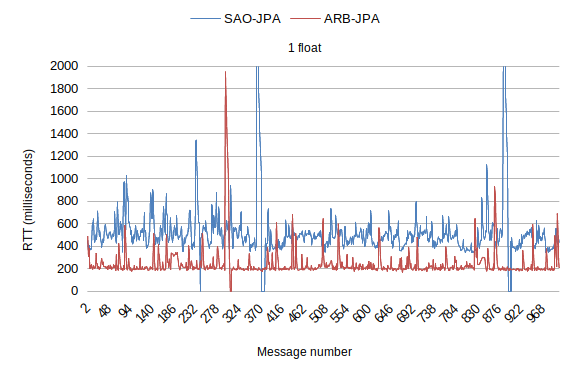
\includegraphics[width=\columnwidth]{z3-d685-c001}
		\caption{One float}
		\label{fig:z3-d685-c001}
	\end{subfigure}
	\begin{subfigure}{.45\textwidth}
		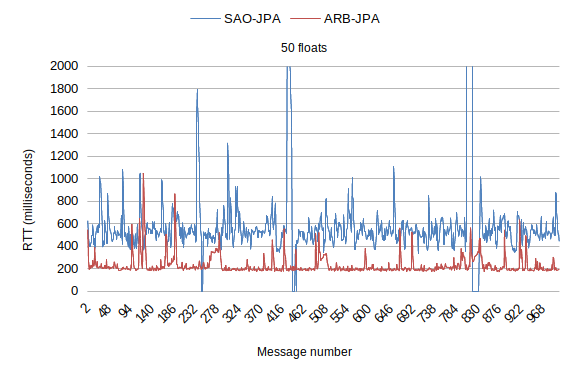
\includegraphics[width=\columnwidth]{z3-d685-c050}
		\caption{50 floats}
		\label{fig:z3-d685-c050}
	\end{subfigure}
	\par\bigskip
	\begin{subfigure}{.45\textwidth}
		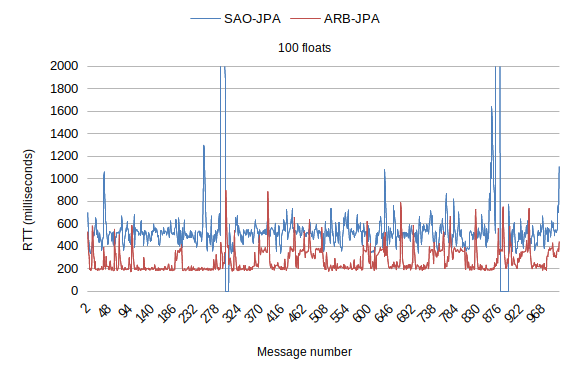
\includegraphics[width=\columnwidth]{z3-d685-c100}
		\caption{100 floats}
		\label{fig:z3-d685-c100}
	\end{subfigure}
	\begin{subfigure}{.45\textwidth}
		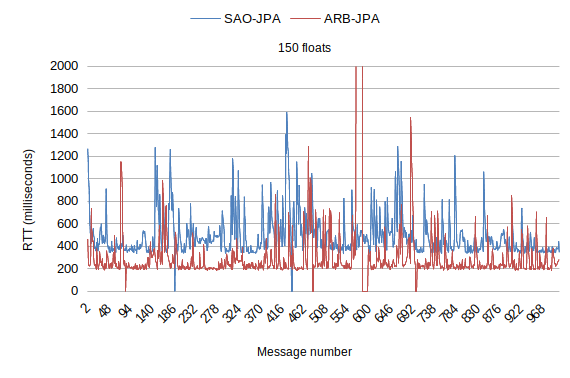
\includegraphics[width=\columnwidth]{z3-d685-c150}
		\caption{150 floats}
		\label{fig:z3-d685-4-c150}
	\end{subfigure}
	\bigskip
	\begin{subfigure}{.45\textwidth}
		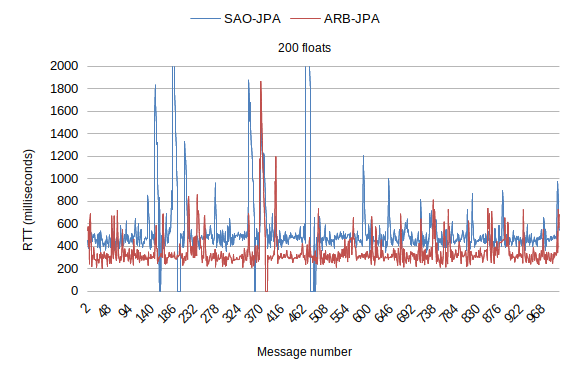
\includegraphics[width=\columnwidth]{z3-d685-c200}
		\caption{200 floats}
		\label{fig:z3-d685-c200}
	\end{subfigure}
	\begin{subfigure}{.45\textwidth}
		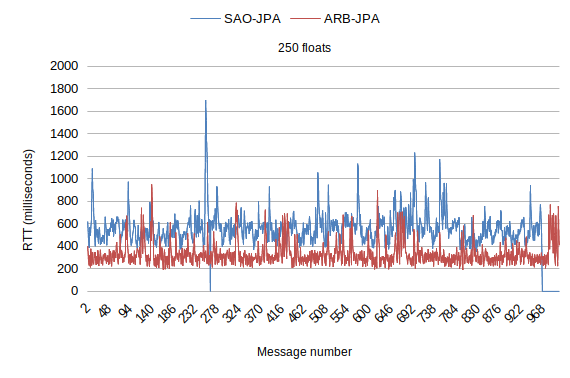
\includegraphics[width=\columnwidth]{z3-d685-c250}
		\caption{250 floats}
		\label{fig:z3-d685-c250}
	\end{subfigure} 
	
	\caption{RTT comparison for different number of floats included in messages sent from São Paulo to João Pessoa~(SAO-JPA) and Ann Arbor to João Pessoa~(ARB-JPA). Lost messages are represented with 0ms RTT. The y-axis maximum is 2000ms for better visualization, but there are some RTTs reaching 4s.}
	\label{fig:z3-d685-evaluation}
\end{figure*}


\begin{table}[]
	\centering
	\begin{tabular}{ll|llllll|}
		&                    & \multicolumn{6}{c|}{Floats per message} \\
		&                    & 1    & 50   & 100  & 150  & 200  & 250  \\ \hline
		\multirow{2}{*}{Message}            & Loss (for 1000)      & 14   & 26   & 25   & 3    & 21   & 38   \\
		& Size (bytes)       & 41   & 614  & 1190 & 1782 & 2355 & 2950 \\ \cline{1-2}
		\multirow{4}{*}{RTT (milliseconds)} & Minimum            & 342  & 332  & 332  & 329  & 332  & 352  \\
		& Maximum            & 2430 & 3916 & 4371 & 1595 & 3014 & 1700 \\
		& Average            & 515  & 578  & 563  & 486  & 536  & 543  \\
		& Standard deviation & 224  & 366  & 394  & 181  & 305  & 168  \\ \hline
	\end{tabular}
	
	\caption{SPA-JPA tests: Results from RTT evaluation using cloud services between S\~{a}o Paulo and Jo\~{a}o Pessoa.}
	\label{tab:sao-jpa}
\end{table}

\begin{table}[]
	\centering
	\begin{tabular}{ll|llllll|}
		&                    & \multicolumn{6}{c|}{Floats per message}  \\
		&                    & 1    & 50   & 100  & 150  & 200  & 250  \\ \hline
		Message             & Loss (for 1000)      & 3    & 0    & 0    & 17   & 5    & 0    \\
		& Size (bytes)       & 43   & 613  & 1189 & 1784 & 2378 & 2935 \\ \cline{1-2}
		RTT (milliseconds) & Minimum            & 166  & 172  & 172  & 182  & 199  & 190  \\
		& Maximum            & 1953 & 1052 & 898  & 3100 & 1869 & 951  \\
		& Average            & 243  & 230  & 273  & 316  & 348  & 329  \\
		& Standard deviation & 138  & 83   & 103  & 317  & 143  & 101  \\ \hline
	\end{tabular}
	
	\caption{ARB-JPA tests: Results from RTT evaluation using cloud services between Ann Arbor and Jo\~{a}o Pessoa.}
	\label{tab:arb-jpa}
\end{table}

We can see in the charts that the RTT is better on ARB-JPA evaluation.
Another point from ARB-JPA evaluation is that the more floats we have on a message, the higher RTT we find.
The SAO-JPA evaluation presented some instability regarding the average RTT and there was no discernible pattern linking the number of floats to the average RTT.
Although we have had some high RTT values during the tests, the concentration of high RTT values appear to be more frequent in clustered sequential messages than when messages are isolated (meaning musical algorithms based on sporadic communication would suffer less). Furthermore, it was relatively common for the service to lose at least one message after a high RTT value.

The results summarized in Table~\ref{tab:sao-jpa} present a minimum RTT of 329ms with 150 floats and average RTT values between 486-578ms for all message sizes.
On the other hand, we have a minimum RTT of 166ms with 1 float in Table~\ref{tab:arb-jpa}, and average RTT values between 230-348ms.
We sent 1000 messages on each test and lost no more than 4\% of the messages in the worst case, and we lost more messages in the SAO-JPA evaluation than in ARB-JPA.
Moreover, ARB-JPA evaluation had tests with zero message loss.
These results are also discussed in the paper presented at Appendix~\ref{ape:papericmc2015}.

%%%%%%%%%%%%%%%%%%%%%%%%%%%%%%%%%%%%%%%%%%%%%%%
\section{Second trial: Delay between packets}
\label{sec:secondtrial}

Based on the results of the first trial we decided to evaluate more services changing the size of the packets.
This evaluation was conducted between Ann Arbor, São Paulo, and João Pessoa in June and July, 2015.
In this case, we evaluated the Pusher and PubNub cloud services regarding their free and paid plans, and we included the Unicast as a reference.
The tables below present the results of the evaluations including these services and the statistical evaluation of the RTT results.
The Pusher paid plan is named pusherP, while the PubNub paid plan is name pubnubP.
At the tables' header, Nobs is the number of observations and when this number is under 1000 it means the we had packet loss during the evaluation.
The size is the number of float numbers inside the packet sent.


\subsection*{Evaluation between São Paulo and João Pessoa} 

The Table~\ref{tab:secondtrialsaojpa} presents the results of RTT evaluation with all the services between São Paulo and João Pessoa.
The results from PubNub were better than the results with the Pusher in most of the cases.
The possible reason is because PubNub presents a cluster in Brazil.
In this case, the packets from PubNub had a shortest path.
The packets sent by Pusher had to travel from São Paulo to USA before coming to João Pessoa, and they also traveled to USA before coming back to São Paulo.

\begin{table}[!htb]
	\small
	\centering
	\caption{Second trial results: RTT evaluation between São Paulo and João Pessoa}
	\label{tab:secondtrialsaojpa}
	\begin{tabular}{llllllllllllll}
		Service    & Size & Delay & Nobs & $\mu$ & $\sigma$  & $\sigma$ \textsuperscript{2} & Skew & Kurt & Min & q1   & q2   & q3   & Max   \\ \midrule
		pubnub     & 1            & 150   & \textbf{999}  & \textbf{2641} & 1436 & 2063440  & 1.64     & 8.04     & \textbf{424} & 1413 & 2471 & 3795 & \textbf{13622} \\
		pubnub     & 50           & 150   & 1000 & 201  & 251  & 63133    & 4.19     & 19.29    & 79  & 110  & 123  & 154  & 1983  \\
		pubnub     & 100          & 150   & 1000 & 187  & 139  & 19391    & 3.66     & 14.90    & 89  & 129  & 145  & 175  & 1155  \\
		pubnub     & 150          & 150   & 1000 & 230  & 359  & 129336   & 7.02     & 55.76    & 99  & 138  & 154  & 188  & 4060  \\
		pubnub     & 200          & 150   & 1000 & 188  & 120  & 14373    & 5.47     & 36.94    & 104 & 143  & 158  & 192  & 1405  \\
		pubnub     & 250          & 150   & 1000 & 196  & 120  & 14517    & 4.53     & 23.56    & 108 & 146  & 166  & 198  & 1228  \\ \hline
		pubnubP & 1            & 150   & \textbf{993}  & 400  & 194  & 37648    & 3.88     & 21.49    & 105 & 303  & 360  & 430  & 2122  \\
		pubnubP & 50           & 150   & 1000 & 143  & 143  & 20451    & 8.11     & 76.99    & 81  & 107  & 115  & 130  & 1917  \\
		pubnubP & 100          & 150   & 1000 & 189  & 227  & 51714    & 5.83     & 39.37    & 86  & 124  & 136  & 156  & 2374  \\
		pubnubP & 150          & 150   & 1000 & 210  & 232  & 54110    & 4.95     & 27.65    & 94  & 137  & 148  & 178  & 2205  \\
		pubnubP & 200          & 150   & 1000 & 238  & 264  & 69520    & 4.21     & 21.17    & 103 & 139  & 156  & 195  & 2368  \\
		pubnubP & 250          & 150   & 1000 & 233  & 251  & 62988    & 5.16     & 31.53    & 108 & 148  & 164  & 200  & 2434  \\ \hline
		pusher     & 1            & 150   & 1000 & 367  & 56   & 3128     & 5.58     & 47.02    & 311 & 341  & 353  & 373  & 1049  \\
		pusher     & 50           & 150   & 1000 & 509  & 135  & 18189    & 0.86     & 1.01     & 321 & 395  & 490  & 603  & 1180  \\
		pusher     & 100          & 150   & 1000 & 490  & 87   & 7626     & 1.01     & 3.80     & 327 & 427  & 487  & 545  & 1047  \\
		pusher     & 150          & 150   & 1000 & 384  & 63   & 3948     & 4.71     & 30.13    & 322 & 355  & 369  & 392  & 939   \\
		pusher     & 200          & 150   & 1000 & 455  & 57   & 3282     & 3.36     & 28.72    & 343 & 426  & 447  & 477  & 1139  \\
		pusher     & 250          & 150   & 1000 & 471  & 82   & 6675     & 4.07     & 34.96    & 341 & 427  & 465  & 499  & 1410  \\ \hline
		pusherP & 1            & 150   & 1000 & 366  & 37   & 1363     & 3.30     & 21.47    & 316 & 344  & 357  & 376  & 759   \\
		pusherP & 50           & 150   & 1000 & 527  & 142  & 20087    & 1.29     & 3.89     & 325 & 416  & 513  & 610  & 1426  \\
		pusherP & 100          & 150   & 1000 & 495  & 92   & 8430     & 1.30     & 6.36     & 332 & 430  & 493  & 549  & 1204  \\
		pusherP & 150          & 150   & 1000 & 385  & 71   & 5097     & 5.71     & 45.45    & 323 & 353  & 369  & 392  & 1205  \\
		pusherP & 200          & 150   & 1000 & 457  & 66   & 4312     & 4.03     & 34.89    & 352 & 423  & 445  & 477  & 1276  \\
		pusherP & 250          & 150   & 1000 & 482  & 85   & 7293     & 3.25     & 23.24    & 346 & 434  & 471  & 518  & 1358  \\ \hline
		unicast & 1            & 150   & 1000 & \textbf{77}   & 47   & 2207     & 11.69    & 157.20   & \textbf{59}  & 68   & 71   & 73   & 860   \\
		unicast & 50           & 150   & \textbf{997}  & 89   & 46   & 2160     & 9.51     & 106.26   & 63  & 79   & 83   & 86   & 722   \\
		unicast & 100          & 150   & \textbf{999}  & 96   & 34   & 1181     & 8.84     & 112.41   & 66  & 84   & 91   & 95   & 664   \\
		unicast & 150          & 150   & \textbf{997}  & 104  & 31   & 989      & 2.79     & 9.90     & 68  & 88   & 94   & 102  & 352   \\
		unicast & 200          & 150   & 1000 & 112  & 51   & 2624     & 7.42     & 89.43    & 68  & 92   & 97   & 108  & 911   \\
		unicast & 250          & 150   & 1000 & 119  & 58   & 3425     & 7.45     & 79.81    & 77  & 96   & 101  & 118  & 948  \\ \bottomrule
	\end{tabular}
\end{table}



\subsection*{Evaluation between Ann Arbor and São Paulo} 

The Table~\ref{tab:secondtrialarbsao} presents the results of RTT evaluation with all the services between Ann Arbor and São Paulo.
In this evaluation the PubNub had RTT higher than expected, even on paid plan.
These results are possible due the Service Layer Agreement~(SLA) of 99.999\% for paid plan users~\footnote{PubNub SLA: \url{https://support.pubnub.com/support/solutions/articles/14000043627-does-pubnub-provide-a-premium-sla-} (visited on December, 2018)}. 
The PubNub and Pusher had similar results between the free and paid plan.
It is assumed that all traffic passed through the same clusters for both plans in this case.

\begin{table}[!htb]
	\footnotesize
	\centering
	\caption{Second trial results: RTT evaluation between Ann Arbor and São Paulo}
	\label{tab:secondtrialarbsao}
	\begin{tabular}{llllllllllllll}
		Service    & Size & Delay & Nobs & $\mu$ & $\sigma$  & $\sigma$ \textsuperscript{2} & Skew & Kurt & Min & q1   & q2   & q3   & Max   \\ \midrule
		pubnub     & 1            & 150   & 1000 & 4486  & 2394 & 5,735,159.30  & -0.32    & -1.09    & 533  & 1785 & 4808  & 6865  & 11925 \\
		pubnub     & 50           & 150   & 1000 & 2802  & 2169 & 4,707,652.22  & 0.66     & -1.40    & 411  & 1184 & 1593  & 5463  & 7452  \\
		pubnub     & 100          & 150   & 1000 & 8373  & 3949 & 15,609,162.36 & -0.22    & -1.18    & 574  & 5002 & 8961  & 12745 & 14132 \\
		pubnub     & 150          & 150   & 1000 & 12413 & 6835 & 46,760,628.81 & 0.06     & -1.28    & 691  & 5632 & 12234 & 18208 & 24622 \\
		pubnub     & 200          & 150   & 1000 & \textbf{15671} & 7297 & 53,303,033.53 & -0.09    & -1.26    & \textbf{2512} & 9251 & 15600 & 22953 & \textbf{27587} \\
		pubnub     & 250          & 150   & 1000 & 12653 & 6277 & 39,441,152.32 & 0.00     & -1.25    & 1710 & 6883 & 12078 & 18890 & 23102 \\ \hline
		pubnubP & 1            & 150   & 1000 & 1001  & 337  & 114,005.71    & 0.79     & -0.24    & 382  & 764  & 926   & 1105  & 1963  \\
		pubnubP & 50           & 150   & 1000 & 2430  & 821  & 675,257.35    & -0.71    & -0.38    & 412  & 1982 & 2588  & 3052  & 3753  \\
		pubnubP & 100          & 150   & 1000 & 9846  & 6167 & 38,072,365.22 & 0.09     & -1.42    & 503  & 3318 & 10591 & 15964 & 19432 \\
		pubnubP & 150          & 150   & 1000 & 9705  & 5531 & 30,620,190.96 & 0.39     & -0.95    & 661  & 4639 & 8725  & 13502 & 19989 \\
		pubnubP & 200          & 150   & 1000 & 12396 & 6090 & 37,121,911.71 & -0.24    & -1.29    & 711  & 7128 & 13680 & 17999 & 21050 \\
		pubnubP & 250          & 150   & \textbf{948}  & 12742 & 7234 & 52,385,134.53 & -0.07    & -1.11    & 697  & 5970 & 14169 & 18398 & 26510 \\ \hline
		pusher     & 1            & 150   & 1000 & 330   & 71   & 5,059.07      & 2.64     & 8.26     & 252  & 292  & 306   & 329   & 756   \\
		pusher     & 50           & 150   & 1000 & 465   & 119  & 14,274.06     & 0.86     & 0.67     & 268  & 383  & 446   & 532   & 938   \\
		pusher     & 100          & 150   & 1000 & 432   & 94   & 8,814.99      & 0.77     & 1.97     & 271  & 348  & 438   & 483   & 984   \\
		pusher     & 150          & 150   & 1000 & 337   & 69   & 4,780.45      & 3.11     & 13.82    & 261  & 297  & 318   & 346   & 922   \\
		pusher     & 200          & 150   & 1000 & 344   & 64   & 4,118.55      & 2.75     & 10.34    & 259  & 307  & 325   & 356   & 777   \\
		pusher     & 250          & 150   & 1000 & 356   & 74   & 5,546.34      & 2.72     & 9.92     & 258  & 313  & 334   & 366   & 873   \\ \hline
		pusherP & 1            & 150   & 1000 & 330   & 69   & 4,833.24      & 2.43     & 7.60     & 251  & 290  & 305   & 342   & 754   \\
		pusherP & 50           & 150   & 1000 & 456   & 113  & 12,726.50     & 0.74     & 0.33     & 255  & 366  & 446   & 514   & 867   \\
		pusherP & 100          & 150   & 1000 & 448   & 86   & 7,480.51      & 0.47     & 1.13     & 264  & 401  & 447   & 498   & 868   \\
		pusherP & 150          & 150   & 1000 & 347   & 107  & 11,495.46     & 5.28     & 35.46    & 261  & 301  & 319   & 348   & 1341  \\
		pusherP & 200          & 150   & 1000 & 338   & 51   & 2,590.98      & 2.33     & 8.29     & 264  & 306  & 324   & 351   & 704   \\
		pusherP & 250          & 150   & 1000 & 364   & 75   & 5,623.51      & 2.09     & 7.04     & 269  & 314  & 337   & 400   & 867   \\ \hline
		unicast & 1            & 150   & 1000 & \textbf{187}   & 38   & 1,425.68      & 4.08     & 19.14    & \textbf{162}  & 173  & 175   & 179   & 457   \\
		unicast & 50           & 150   & \textbf{998}  & 196   & 34   & 1,162.23      & 4.23     & 20.61    & 167  & 183  & 188   & 191   & 458   \\
		unicast & 100          & 150   & \textbf{999}  & 204   & 33   & 1,101.55      & 4.62     & 26.92    & 171  & 191  & 197   & 202   & 503   \\
		unicast & 150          & 150   & \textbf{999}  & 215   & 46   & 2,079.68      & 7.26     & 99.10    & 174  & 196  & 204   & 210   & 1013  \\
		unicast & 200          & 150   & 1000 & 224   & 42   & 1,732.19      & 3.07     & 12.20    & 175  & 203  & 211   & 221   & 511   \\
		unicast & 250          & 150   & \textbf{999}  & 233   & 52   & 2,748.36      & 5.65     & 65.50    & 178  & 208  & 217   & 231   & 1058 \\ \bottomrule
	\end{tabular}
\end{table} 


\subsection*{Evaluation between Ann Arbor and João Pessoa} 

The Table~\ref{tab:secondtrialarbjpa} presents the results of RTT evaluation with all the services between Ann Arbor and João Pessoa.
The results of this evaluation presented similar values between Pusher and Unicast, which were unexpected.
The possible reason is that the packets sent using Unicast were passing by São Paulo PoP instead of Fortaleza PoP, which is the closest to US.
At the same time, packets sent using Pusher can follow routes outside the academic network before reaching the clusters.

\begin{table}[!htb]
	\small
	\centering
	\caption{Second trial results: RTT evaluation between Ann Arbor and João Pessoa}
	\label{tab:secondtrialarbjpa}
	\begin{tabular}{llllllllllllll}
		Service    & Size & Delay & Nobs & $\mu$ & $\sigma$  & $\sigma$ \textsuperscript{2} & Skew & Kurt & Min & q1   & q2   & q3   & Max   \\ \midrule
		pubnub     & 1            & 150   & 1000 & 480  & 298  & 89,045.38    & 4.92     & 26.81    & 364 & 383 & 394 & 420 & 2905  \\
		pubnub     & 50           & 150   & 1000 & 498  & 400  & 160,061.26   & 9.02     & 107.13   & 367 & 391 & 404 & 432 & 6737  \\
		pubnub     & 100          & 150   & 1000 & 493  & 447  & 199,905.79   & 10.21    & 123.85   & 373 & 405 & 418 & 439 & 7243  \\
		pubnub     & 150          & 150   & 1000 & 642  & 554  & 307,458.81   & 7.39     & 64.52    & 461 & 504 & 519 & 558 & 7237  \\
		pubnub     & 200          & 150   & 1000 & 661  & 597  & 356,749.09   & 5.39     & 31.07    & 461 & 488 & 513 & 549 & 5410  \\
		pubnub     & 250          & 150   & 1000 & 845  & 1863 & 3,475,934.57 & 9.46     & 95.36    & 471 & 522 & 548 & 609 & \textbf{25559} \\ \hline
		pubnubP & 1            & 150   & 1000 & 497  & 437  & 191,571.06   & 8.31     & 88.06    & 357 & 382 & 391 & 421 & 6618  \\
		pubnubP & 50           & 150   & 1000 & 486  & 351  & 123,638.71   & 8.82     & 98.78    & 366 & 389 & 400 & 428 & 5237  \\
		pubnubP & 100          & 150   & 1000 & 566  & 834  & 696,442.12   & 10.98    & 142.63   & 374 & 406 & 420 & 452 & 13930 \\
		pubnubP & 150          & 150   & 1000 & 573  & 370  & 136,770.67   & 12.47    & 179.77   & 462 & 503 & 516 & 541 & 7120  \\
		pubnubP & 200          & 150   & 1000 & 666  & 401  & 160,645.05   & 3.76     & 15.15    & 463 & 511 & 530 & 599 & 3768  \\
		pubnubP & 250          & 150   & 1000 & 635  & 293  & 86,179.32    & 3.79     & 16.20    & 471 & 517 & 535 & 583 & 2756  \\ \hline
		pusher     & 1            & 150   & 1000 & \textbf{209}  & 32   & 1,012.05     & 4.24     & 27.14    & \textbf{170} & 192 & 205 & 215 & 503   \\
		pusher     & 50           & 150   & 1000 & 217  & 36   & 1,296.08     & 3.59     & 18.62    & 174 & 198 & 210 & 222 & 550   \\
		pusher     & 100          & 150   & 1000 & 233  & 58   & 3,347.10     & 6.20     & 64.38    & 172 & 206 & 217 & 242 & 1015  \\
		pusher     & 150          & 150   & 1000 & 234  & 77   & 5,973.63     & 6.04     & 44.86    & 177 & 203 & 218 & 232 & 1059  \\
		pusher     & 200          & 150   & 1000 & 306  & 46   & 2,103.95     & 1.10     & 5.66     & 201 & 279 & 303 & 334 & 654   \\
		pusher     & 250          & 150   & \textbf{995}  & 336  & 157  & 24,688.01    & 7.57     & 73.07    & 190 & 273 & 320 & 356 & 2243  \\ \hline
		pusherP & 1            & 150   & 1000 & 213  & 62   & 3,850.73     & 7.65     & 75.03    & 171 & 190 & 202 & 216 & 976   \\
		pusherP & 50           & 150   & 1000 & 222  & 37   & 1,380.66     & 3.56     & 21.20    & 173 & 201 & 213 & 227 & 598   \\
		pusherP & 100          & 150   & \textbf{999}  & 250  & 95   & 9,124.09     & 5.80     & 51.87    & 177 & 206 & 220 & 256 & 1387  \\
		pusherP & 150          & 150   & 1000 & 225  & 29   & 861.74       & 1.81     & 4.50     & 180 & 207 & 219 & 233 & 387   \\
		pusherP & 200          & 150   & \textbf{980}  & 396  & 783  & 613,390.44   & 8.89     & 77.74    & 194 & 278 & 307 & 339 & 8187  \\
		pusherP & 250          & 150   & 1000 & 319  & 55   & 3,033.88     & -0.01    & -0.15    & 199 & 283 & 323 & 356 & 561   \\ \hline
		unicast & 1            & 150   & 1000 & 231  & 15   & 230.51       & 9.71     & 106.79   & 222 & 228 & 229 & 231 & 427   \\
		unicast & 50           & 150   & 1000 & 242  & 24   & 560.52       & 8.36     & 88.98    & 225 & 235 & 239 & 243 & 611   \\
		unicast & 100          & 150   & 1000 & 250  & 35   & 1,252.13     & 11.92    & 183.23   & 226 & 241 & 245 & 251 & 915   \\
		unicast & 150          & 150   & 1000 & 259  & 37   & 1,351.90     & 4.93     & 29.33    & 232 & 245 & 250 & 258 & 595   \\
		unicast & 200          & 150   & 1000 & 260  & 41   & 1,713.40     & 10.96    & 146.77   & 234 & 248 & 254 & 263 & 973   \\
		unicast & 250          & 150   & 1000 & 268  & 36   & 1,281.82     & 8.06     & 98.89    & 238 & 253 & 260 & 271 & 851  \\ \bottomrule
	\end{tabular}
\end{table}






%%%%%%%%%%%%%%%%%%%%%%%%%%%%%%%%%%%%%%%%%%%%%%%%%%%%%%%%%%%%%%%%%%%%%%%
\section{Third trial: IPv4 versus IPv6}
\label{sec:thirdtrial}

The Table~\ref{tab:thirdtrialarbsaoipv4} and Table~\ref{tab:thirdtrialarbsaoipv6} present the results of RTT evaluation with Unicast through IPv4 and IPv6 protocols between Ann Arbor and São Paulo.
This evaluation was conducted on February, 2017, due to many technical reasons.
We spent more than one year trying to setup the Multicast between RNP and Internet2, but the service was unstable all the time.
The network managers did their best, but in the end we decided to abort the evaluation due to time limit constraints to finish this thesis.

In the end, the evaluation with on IPv4 and IPv6 had interesting results.
IPv6 seems to offer fastest paths than IPv4, although IPv4 presents less packet loss.
The packet loss was present in all evaluations with IPv6 and the possible reason for this situation is that the protocol is still being implemented and evaluated at some paths of the academic network.
Another possible reason is that some devices may not work properly with this protocol yet.


\begin{table}[!htb]
	\small
	\centering
	\caption{Third trial results: IPv4 RTT evaluation between Ann Arbor and São Paulo}
	\label{tab:thirdtrialarbsaoipv4}
	\begin{tabular}{@{}llllllllllllll@{}}
		\toprule
		Service    & Size & Delay & Nobs & $\mu$ & $\sigma$  & $\sigma$ \textsuperscript{2} & Skew & Kurt & Min & q1   & q2   & q3   & Max   \\ \midrule
		unicastIPv4 & 2            & 2     & 1000 & 217  & 60  & 3,558.09 & 1.14     & 0.46     & 165 & 170 & 186 & 256 & 450  \\
		unicastIPv4 & 2            & 4     & 1000 & \textbf{209}  & 53  & 2,793.07 & 1.28     & 0.85     & \textbf{164} & 170 & 175 & 243 & 412  \\
		unicastIPv4 & 2            & 8     & 1000 & 216  & 58  & 3,356.04 & 1.22     & 1.13     & \textbf{164} & 170 & 186 & 256 & 488  \\
		unicastIPv4 & 2            & 16    & 1000 & 214  & 55  & 3,013.90 & 1.14     & 0.42     & \textbf{164} & 171 & 183 & 252 & 417  \\
		unicastIPv4 & 2            & 32    & 1000 & 212  & 57  & 3,291.98 & 1.62     & 2.27     & 166 & 174 & 180 & 241 & 477  \\
		unicastIPv4 & 2            & 64    & 1000 & 221  & 56  & 3,133.15 & 1.31     & 1.07     & 167 & 181 & 190 & 252 & 431  \\
		unicastIPv4 & 2            & 128   & 1000 & 222  & 59  & 3,518.46 & 1.45     & 1.96     & 167 & 181 & 185 & 261 & 502  \\ \hline
		unicastIPv4 & 4            & 2     & 1000 & 224  & 60  & 3,632.01 & 1.04     & 0.63     & \textbf{164} & 171 & 205 & 265 & 491  \\
		unicastIPv4 & 4            & 4     & \textbf{999}  & 214  & 57  & 3,300.74 & 1.21     & 0.68     & \textbf{164} & 170 & 180 & 251 & 443  \\
		unicastIPv4 & 4            & 8     & 1000 & 215  & 58  & 3,337.70 & 1.29     & 1.35     & \textbf{164} & 170 & 185 & 251 & 511  \\
		unicastIPv4 & 4            & 16    & 1000 & 211  & 56  & 3,111.82 & 1.51     & 1.94     & 165 & 171 & 178 & 243 & 503  \\
		unicastIPv4 & 4            & 32    & 1000 & 219  & 58  & 3,347.05 & 1.24     & 0.93     & 166 & 175 & 186 & 257 & 492  \\
		unicastIPv4 & 4            & 64    & 1000 & 224  & 59  & 3,524.73 & 1.48     & 2.03     & 167 & 182 & 193 & 257 & 507  \\
		unicastIPv4 & 4            & 128   & 1000 & 220  & 58  & 3,418.48 & 1.52     & 1.92     & 166 & 182 & 185 & 252 & 491  \\ \hline
		unicastIPv4 & 8            & 2     & 1000 & 216  & 61  & 3,668.89 & 1.31     & 1.00     & \textbf{164} & 171 & 178 & 251 & 485  \\
		unicastIPv4 & 8            & 4     & 1000 & 213  & 60  & 3,655.43 & 1.56     & 2.05     & 165 & 171 & 176 & 245 & 491  \\
		unicastIPv4 & 8            & 8     & 1000 & 219  & 61  & 3,707.13 & 1.32     & 1.45     & 166 & 171 & 184 & 258 & 513  \\
		unicastIPv4 & 8            & 16    & 1000 & 213  & 58  & 3,423.24 & 1.46     & 1.49     & 165 & 172 & 178 & 247 & 482  \\
		unicastIPv4 & 8            & 32    & 1000 & 224  & 60  & 3,641.28 & 1.29     & 1.38     & 166 & 176 & 197 & 259 & 493  \\
		unicastIPv4 & 8            & 64    & 1000 & 222  & 57  & 3,201.64 & 1.52     & 2.14     & 166 & 182 & 191 & 253 & 497  \\
		unicastIPv4 & 8            & 128   & 1000 & 226  & 63  & 3,992.91 & 1.63     & 2.79     & 169 & 183 & 187 & 263 & 535  \\ \hline
		unicastIPv4 & 16           & 2     & 1000 & 214  & 57  & 3,207.92 & 1.32     & 1.00     & 166 & 173 & 178 & 250 & 460  \\
		unicastIPv4 & 16           & 4     & 1000 & 216  & 55  & 3,031.27 & 1.14     & 0.39     & 165 & 173 & 182 & 255 & 420  \\
		unicastIPv4 & 16           & 8     & 1000 & 214  & 55  & 3,047.55 & 1.30     & 1.04     & 165 & 173 & 180 & 251 & 458  \\
		unicastIPv4 & 16           & 16    & 1000 & 227  & 63  & 4,021.29 & 1.18     & 0.79     & 166 & 175 & 198 & 265 & 489  \\
		unicastIPv4 & 16           & 32    & 1000 & 221  & 57  & 3,295.46 & 1.35     & 1.54     & 166 & 178 & 188 & 255 & 516  \\
		unicastIPv4 & 16           & 64    & 1000 & 223  & 54  & 2,879.77 & 1.37     & 1.31     & 168 & 185 & 192 & 254 & 456  \\
		unicastIPv4 & 16           & 128   & 1000 & 232  & 66  & 4,318.96 & 1.41     & 1.64     & 166 & 185 & 192 & 273 & 509  \\ \hline
		unicastIPv4 & 32           & 2     & 1000 & 222  & 58  & 3,392.14 & 1.17     & 0.71     & 167 & 177 & 188 & 264 & 469  \\
		unicastIPv4 & 32           & 4     & 1000 & 227  & 58  & 3,348.27 & 0.99     & 0.37     & 166 & 177 & 203 & 269 & 497  \\
		unicastIPv4 & 32           & 8     & 1000 & 224  & 62  & 3,873.42 & 1.40     & 1.71     & 166 & 177 & 189 & 262 & 497  \\
		unicastIPv4 & 32           & 16    & 1000 & 226  & 62  & 3,820.62 & 1.38     & 1.73     & 168 & 178 & 193 & 264 & 550  \\
		unicastIPv4 & 32           & 32    & 1000 & 221  & 57  & 3,221.42 & 1.50     & 2.08     & 166 & 181 & 190 & 254 & 518  \\
		unicastIPv4 & 32           & 64    & 1000 & 228  & 55  & 3,013.00 & 1.50     & 2.25     & 166 & 189 & 199 & 260 & 517  \\
		unicastIPv4 & 32           & 128   & 1000 & 230  & 61  & 3,728.85 & 1.55     & 2.32     & 170 & 188 & 194 & 267 & 511  \\ \hline
		unicastIPv4 & 64           & 2     & 1000 & 230  & 59  & 3,540.37 & 1.20     & 1.06     & 168 & 183 & 199 & 272 & 487  \\
		unicastIPv4 & 64           & 4     & 1000 & 234  & 58  & 3,386.02 & 0.94     & 0.13     & 168 & 184 & 215 & 275 & 478  \\
		unicastIPv4 & 64           & 8     & 1000 & 232  & 60  & 3,573.38 & 1.08     & 0.55     & 169 & 184 & 208 & 274 & 495  \\
		unicastIPv4 & 64           & 16    & 1000 & 232  & 59  & 3,513.60 & 1.30     & 1.41     & 171 & 186 & 200 & 271 & 506  \\
		unicastIPv4 & 64           & 32    & 1000 & 238  & 70  & 4,884.21 & 1.48     & 1.85     & 169 & 187 & 200 & 273 & 518  \\
		unicastIPv4 & 64           & 64    & 1000 & 234  & 53  & 2,818.47 & 1.26     & 0.84     & 172 & 196 & 207 & 264 & 454  \\
		unicastIPv4 & 64           & 128   & 1000 & 237  & 59  & 3,430.93 & 1.43     & 2.20     & 168 & 194 & 204 & 276 & 559  \\ \hline
		unicastIPv4 & 128          & 2     & 1000 & 246  & 68  & 4,618.75 & 1.49     & 3.63     & 172 & 192 & 220 & 293 & \textbf{673}  \\
		unicastIPv4 & 128          & 4     & 1000 & 246  & 61  & 3,681.45 & 0.92     & 0.32     & 172 & 193 & 227 & 291 & 521  \\
		unicastIPv4 & 128          & 8     & 1000 & 237  & 61  & 3,677.11 & 1.32     & 1.42     & 174 & 192 & 206 & 276 & 511  \\
		unicastIPv4 & 128          & 16    & 1000 & 241  & 60  & 3,608.68 & 1.18     & 1.02     & 175 & 193 & 215 & 279 & 491  \\
		unicastIPv4 & 128          & 32    & 1000 & 241  & 59  & 3,498.73 & 1.31     & 1.57     & 174 & 195 & 213 & 279 & 537  \\
		unicastIPv4 & 128          & 64    & 1000 & 246  & 62  & 3,897.96 & 1.72     & 3.65     & 178 & 203 & 216 & 278 & 640  \\
		unicastIPv4 & 128          & 128   & 1000 & 245  & 64  & 4,084.91 & 1.59     & 2.39     & 179 & 201 & 213 & 278 & 527  \\ \bottomrule
	\end{tabular}
\end{table}



\begin{table}[!htb]
	\centering
	\caption{Third trial results: IPv6 RTT evaluation between Ann Arbor and São Paulo}
	\label{tab:thirdtrialarbsaoipv6}
	\begin{tabular}{@{}llllllllllllll@{}}
		\toprule
		Service    & Size & Delay & Nobs & $\mu$ & $\sigma$  & $\sigma$ \textsuperscript{2} & Skew & Kurt & Min & q1   & q2   & q3   & Max   \\ \midrule
		unicastIPv6 & 2            & 2     & \textbf{931}  & 209  & 83  & 6,899.31 & 11.95    & 251.88   & 162 & 166 & 171 & 241 & \textbf{2040} \\
		unicastIPv6 & 2            & 4     & \textbf{981}  & 213  & 61  & 3,780.19 & 1.38     & 1.60     & \textbf{161} & 167 & 176 & 250 & 512  \\
		unicastIPv6 & 2            & 8     & \textbf{966}  & \textbf{207}  & 56  & 3,142.12 & 1.35     & 1.18     & \textbf{161} & 167 & 172 & 243 & 470  \\
		unicastIPv6 & 2            & 16    & \textbf{977}  & 219  & 59  & 3,508.90 & 1.04     & 0.27     & \textbf{161} & 168 & 194 & 259 & 460  \\
		unicastIPv6 & 2            & 32    & \textbf{987}  & 218  & 56  & 3,165.50 & 1.16     & 1.02     & 162 & 172 & 194 & 255 & 505  \\
		unicastIPv6 & 2            & 64    & \textbf{990}  & 224  & 61  & 3,664.21 & 1.35     & 1.53     & 162 & 178 & 198 & 257 & 487  \\
		unicastIPv6 & 2            & 128   & \textbf{986}  & 216  & 56  & 3,093.35 & 1.54     & 2.21     & 164 & 178 & 184 & 248 & 508  \\ \hline
		unicastIPv6 & 4            & 2     & \textbf{976}  & 210  & 60  & 3,637.20 & 1.47     & 1.75     & \textbf{161} & 167 & 172 & 244 & 502  \\
		unicastIPv6 & 4            & 4     & \textbf{977}  & 210  & 58  & 3,361.79 & 1.37     & 1.39     & 162 & 167 & 173 & 246 & 495  \\
		unicastIPv6 & 4            & 8     & \textbf{975}  & 211  & 57  & 3,247.00 & 1.24     & 0.84     & 162 & 167 & 177 & 248 & 447  \\
		unicastIPv6 & 4            & 16    & \textbf{981}  & 214  & 61  & 3,684.01 & 1.45     & 1.88     & \textbf{161} & 168 & 179 & 247 & 493  \\
		unicastIPv6 & 4            & 32    & \textbf{979}  & 213  & 57  & 3,248.35 & 1.35     & 1.09     & 162 & 172 & 179 & 247 & 459  \\
		unicastIPv6 & 4            & 64    & \textbf{978}  & 217  & 58  & 3,323.11 & 1.73     & 3.37     & 164 & 178 & 186 & 246 & 506  \\
		unicastIPv6 & 4            & 128   & \textbf{975}  & 222  & 64  & 4,120.21 & 1.63     & 2.48     & 164 & 179 & 183 & 256 & 498  \\ \hline
		unicastIPv6 & 8            & 2     & \textbf{972}  & 214  & 60  & 3,565.14 & 1.29     & 1.35     & 162 & 168 & 179 & 252 & 513  \\
		unicastIPv6 & 8            & 4     & \textbf{982}  & 217  & 59  & 3,525.46 & 1.17     & 0.73     & \textbf{161} & 168 & 187 & 255 & 470  \\
		unicastIPv6 & 8            & 8     & \textbf{983}  & 216  & 68  & 4,617.50 & 1.62     & 2.39     & 162 & 168 & 174 & 249 & 506  \\
		unicastIPv6 & 8            & 16    & \textbf{983}  & 218  & 62  & 3,812.69 & 1.39     & 1.81     & 162 & 170 & 190 & 254 & 506  \\
		unicastIPv6 & 8            & 32    & \textbf{974}  & 217  & 60  & 3,643.81 & 1.48     & 1.97     & 162 & 173 & 182 & 251 & 502  \\
		unicastIPv6 & 8            & 64    & \textbf{974}  & 216  & 53  & 2,818.20 & 1.42     & 1.50     & 164 & 180 & 186 & 247 & 440  \\
		unicastIPv6 & 8            & 128   & \textbf{974}  & 220  & 57  & 3,205.65 & 1.36     & 1.32     & 164 & 180 & 185 & 254 & 496  \\ \hline
		unicastIPv6 & 16           & 2     & \textbf{983}  & 214  & 56  & 3,186.99 & 1.17     & 0.46     & 162 & 170 & 180 & 248 & 417  \\
		unicastIPv6 & 16           & 4     & \textbf{979}  & 214  & 58  & 3,402.94 & 1.23     & 0.71     & 162 & 170 & 178 & 253 & 453  \\
		unicastIPv6 & 16           & 8     & \textbf{976}  & 213  & 56  & 3,094.19 & 1.24     & 0.73     & 163 & 171 & 179 & 249 & 419  \\
		unicastIPv6 & 16           & 16    & \textbf{976}  & 215  & 60  & 3,547.88 & 1.45     & 1.81     & 163 & 171 & 181 & 251 & 502  \\
		unicastIPv6 & 16           & 32    & \textbf{978}  & 218  & 60  & 3,577.64 & 1.50     & 1.99     & 164 & 175 & 183 & 251 & 496  \\
		unicastIPv6 & 16           & 64    & \textbf{971}  & 224  & 58  & 3,334.72 & 1.34     & 1.37     & 166 & 181 & 194 & 258 & 478  \\
		unicastIPv6 & 16           & 128   & \textbf{976}  & 223  & 60  & 3,634.23 & 1.61     & 2.68     & 166 & 182 & 187 & 259 & 517  \\ \hline
		unicastIPv6 & 32           & 2     & \textbf{978}  & 215  & 56  & 3,137.36 & 1.30     & 1.10     & 165 & 174 & 182 & 253 & 481  \\
		unicastIPv6 & 32           & 4     & \textbf{969}  & 216  & 58  & 3,374.93 & 1.29     & 0.79     & 164 & 174 & 181 & 252 & 459  \\
		unicastIPv6 & 32           & 8     & \textbf{973}  & 216  & 58  & 3,338.28 & 1.30     & 1.07     & 163 & 173 & 181 & 253 & 476  \\
		unicastIPv6 & 32           & 16    & \textbf{973}  & 223  & 59  & 3,505.97 & 1.23     & 1.08     & 164 & 176 & 193 & 261 & 482  \\
		unicastIPv6 & 32           & 32    & \textbf{966}  & 222  & 57  & 3,278.71 & 1.28     & 1.05     & 165 & 179 & 190 & 257 & 470  \\
		unicastIPv6 & 32           & 64    & \textbf{972}  & 229  & 57  & 3,201.44 & 1.33     & 1.38     & 169 & 187 & 200 & 262 & 497  \\
		unicastIPv6 & 32           & 128   & \textbf{968}  & 229  & 58  & 3,425.28 & 1.31     & 1.14     & 168 & 186 & 194 & 264 & 486  \\ \hline
		unicastIPv6 & 64           & 2     & \textbf{975}  & 226  & 60  & 3,619.86 & 1.21     & 0.94     & 165 & 180 & 191 & 265 & 483  \\
		unicastIPv6 & 64           & 4     & \textbf{981}  & 225  & 59  & 3,535.05 & 1.24     & 1.06     & 166 & 180 & 191 & 265 & 487  \\
		unicastIPv6 & 64           & 8     & \textbf{974}  & 223  & 60  & 3,615.61 & 1.45     & 1.88     & 166 & 180 & 189 & 259 & 515  \\
		unicastIPv6 & 64           & 16    & \textbf{983}  & 226  & 59  & 3,542.56 & 1.36     & 1.68     & 167 & 182 & 194 & 265 & 514  \\
		unicastIPv6 & 64           & 32    & \textbf{982}  & 226  & 58  & 3,396.10 & 1.61     & 2.96     & 166 & 184 & 195 & 261 & 523  \\
		unicastIPv6 & 64           & 64    & \textbf{975}  & 233  & 59  & 3,536.28 & 1.69     & 3.14     & 167 & 191 & 204 & 262 & 516  \\
		unicastIPv6 & 64           & 128   & \textbf{976}  & 239  & 64  & 4,159.53 & 1.60     & 3.15     & 173 & 192 & 205 & 277 & 621  \\ \hline
		unicastIPv6 & 128          & 2     & \textbf{972}  & 243  & 66  & 4,323.65 & 1.10     & 0.85     & 169 & 188 & 216 & 288 & 535  \\
		unicastIPv6 & 128          & 4     & \textbf{962}  & 233  & 59  & 3,471.90 & 1.18     & 0.81     & 170 & 188 & 201 & 273 & 488  \\
		unicastIPv6 & 128          & 8     & \textbf{970}  & 246  & 79  & 6,213.39 & 1.46     & 1.69     & 169 & 187 & 202 & 286 & 576  \\
		unicastIPv6 & 128          & 16    & \textbf{964}  & 239  & 59  & 3,519.94 & 1.08     & 0.50     & 171 & 192 & 209 & 280 & 474  \\
		unicastIPv6 & 128          & 32    & \textbf{966}  & 234  & 54  & 2,971.64 & 1.18     & 0.65     & 171 & 193 & 206 & 270 & 444  \\
		unicastIPv6 & 128          & 64    & \textbf{976}  & 235  & 51  & 2,578.85 & 1.37     & 1.40     & 173 & 200 & 211 & 263 & 481  \\
		unicastIPv6 & 128          & 128   & \textbf{980}  & 240  & 59  & 3,486.10 & 1.52     & 2.27     & 175 & 199 & 209 & 275 & 531  \\ \bottomrule
	\end{tabular}
\end{table}




